%
% reelle-beispiele.tex -- Reelle Beispiele und Gegenbeispiele
%
% !TEX root = ../../buch.tex
% !TEX encoding = UTF-8
%
\section{Reelle Beispiele und Gegenbeispiele
\label{hauptwert:section:reelle-beispiele}}
\kopfrechts{Reelle Beispiele}

\subsection{Ein weiteres Beispiel in der reellen Analysis}
%
% nichtungerade.tex
%
% (c) 2026 Damien Flury, OST Ostschweizer Fachhochschule
%
\begin{figure}
\centering
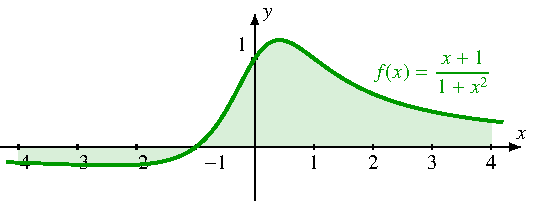
\includegraphics{papers/hauptwert/images/nichtungerade.pdf}
\caption{Graph der Funktion $f(x)=(x+1)/(1+x^2)$.
Der Integrand ist weder gerade noch ungerade;
bei symmetrischer Integration hebt sich nur sein ungerader Anteil weg.
\label{hauptwert:figure:nichtungerade}}
\end{figure}

Als zweites Beispiel betrachten wir die Funktion $f(x) = \frac{x + 1}{1 + x^2}$
und deren uneigentliches Integral $\int_{-\infty}^{\infty} \frac{x + 1}{1 + x^2}\,dx$.
Abbildung \ref{hauptwert:figure:nichtungerade} zeigt den Graphen des Integranden.
Versucht man wieder asymmetrisch von $-\infty$ nach $\infty$ zu integrieren,
erhält man
\begin{equation}
\begin{aligned}
  \int_{-\infty}^{\infty} \frac{x + 1}{1 + x^2}\,dx
  &= \int_{-\infty}^{\infty}
     \biggl(\frac{x}{1 + x^2} + \frac{1}{1 + x^2}\biggr)\,dx \\
  &= \Bigl[\tfrac{1}{2}\ln(1 + x^2) + \arctan x\Bigr]_{-\infty}^{\infty} \\
  &= \lim_{x\to\infty} \Bigl(\tfrac{1}{2}\ln(1 + x^2) + \arctan x\Bigr)
   - \lim_{x\to-\infty} \Bigl(\tfrac{1}{2}\ln(1 + x^2) + \arctan x\Bigr),
\end{aligned}
\end{equation}
also wieder den unbestimmten Ausdruck $\infty - \infty$.
Das uneigentliche Integral existiert also nicht.
Da der Integrand aber wieder ungerade ist, liefert die symmetrische
Annäherung nach Cauchy den Hauptwert
\begin{equation}
\begin{aligned}
  \pv \int_{-\infty}^{\infty} \frac{x + 1}{1 + x^2}\,dx
  &= \lim_{R\to\infty}
     \Bigl[\tfrac{1}{2}\ln(1 + x^2) + \arctan x\Bigr]_{-R}^{R} \\
  &= \lim_{R\to\infty} 2\arctan R \\
  &= \pi.
\end{aligned}
\end{equation}

\subsection{Eine Polstelle im Innern des Intervalls
\label{hauptwert:subsection:pol-innen}}
%
% pol-innen.tex
%
% (c) 2026 Damien Flury, OST Ostschweizer Fachhochschule
%
\begin{figure}
\centering
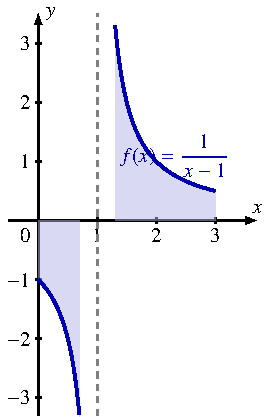
\includegraphics{papers/hauptwert/images/pol-innen.pdf}
\caption{Graph der Funktion $f(x)=1/(x-1)$ auf $[0,3]$.
Die Polstelle bei $x=1$ liegt im Innern des Integrationsintervalls;
symmetrische Annäherung mit gemeinsamem $\varepsilon$ liefert den Hauptwert.
\label{hauptwert:figure:pol-innen}}
\end{figure}

Beim Integral von $1/x$ über $\mathbb{R}$ traten beide Arten von Divergenz
gleichzeitig auf, im vorherigen Beispiel lag sie allein an den unendlichen
Integrationsgrenzen.
Es bleibt der dritte Fall, in dem das Integrationsintervall beschränkt ist
und einzig die Polstelle im Innern regularisiert werden muss.
Dazu dient die Funktion $f(x) = \frac{1}{x - 1}$ auf dem Intervall $[0,3]$,
deren Graph in Abbildung~\ref{hauptwert:figure:pol-innen} dargestellt ist.
Während man beim unendlichen Integral von
$f(x) = \frac{1}{x}$ möglicherweise eine gewisse Symmetrie entdecken konnte und
$0$ hätte erraten können, ist dies hier nicht mehr selbstverständlich.
Die Polstelle liegt bei $x = 1$ und teilt das Intervall in zwei verschieden
lange Teilintervalle, die symmetrische Annäherung bezieht sich also auf die
Polstelle und nicht auf das Intervall.
Nach Definition~\ref{hauptwert:definition:pol} nähert man sich der Polstelle
von beiden Seiten mit einem gemeinsamen $\varepsilon$ und erhält
\begin{equation}
\begin{aligned}
\pv\int_0^3 \frac{dx}{x-1}
  &= \lim_{\varepsilon \to 0^+}
     \biggl(
     \int_{0}^{1 - \varepsilon} \frac{dx}{x - 1} + \int_{1 + \varepsilon}^{3} \frac{dx}{x - 1}
     \biggr) \\
  &= \lim_{\varepsilon \to 0^+}
     \Bigl(\bigl[\ln|x - 1|\bigr]_{0}^{1 - \varepsilon} + \bigl[\ln|x - 1|\bigr]_{1 + \varepsilon}^{3}\Bigr) \\
  &= \lim_{\varepsilon \to 0^+} \bigl(\ln\varepsilon - \ln 1 + \ln 2 - \ln\varepsilon\bigr) \\
  &= \ln 2.
\end{aligned}
\label{hauptwert:equation:beispiel-pol-innen}
\end{equation}
Die beiden Terme $\ln\varepsilon$ heben sich in
\eqref{hauptwert:equation:beispiel-pol-innen} gerade weg,
weil das gemeinsame $\varepsilon$ die Polstelle von beiden Seiten
gleich schnell erreicht.
Übrig bleibt der endliche Wert $\ln 2$, obwohl das uneigentliche Integral
mit zwei unabhängigen Grenzwerten nicht existiert.
